%%%%%%%%%%%%%%%%%%%%%%%%%%%%%%%%%%%%%%%%%
% Beamer Presentation
% LaTeX Template
% Version 1.0 (10/11/12)
%
% This template has been downloaded from:
% http://www.LaTeXTemplates.com
%
% License:
% CC BY-NC-SA 3.0 (http://creativecommons.org/licenses/by-nc-sa/3.0/)
%
%%%%%%%%%%%%%%%%%%%%%%%%%%%%%%%%%%%%%%%%%

%----------------------------------------------------------------------------------------
%	PACKAGES AND THEMES
%----------------------------------------------------------------------------------------

\documentclass{beamer}

\mode<presentation> {

% The Beamer class comes with a number of default slide themes
% which change the colors and layouts of slides. Below this is a list
% of all the themes, uncomment each in turn to see what they look like.

%\usetheme{default}
%\usetheme{AnnArbor}
%\usetheme{Antibes}
%\usetheme{Bergen}
%\usetheme{Berkeley}
%\usetheme{Berlin}
\usetheme{Boadilla}
%\usetheme{CambridgeUS}
%\usetheme{Copenhagen}
%\usetheme{Darmstadt}
%\usetheme{Dresden}
%\usetheme{Frankfurt}
%\usetheme{Goettingen}
%\usetheme{Hannover}
%\usetheme{Ilmenau}
%\usetheme{JuanLesPins}
%\usetheme{Luebeck}
%\usetheme{Madrid}
%\usetheme{Malmoe}
%\usetheme{Marburg}
%\usetheme{Montpellier}
%\usetheme{PaloAlto}
%\usetheme{Pittsburgh}
%\usetheme{Rochester}
%\usetheme{Singapore}
%\usetheme{Szeged}
%\usetheme{Warsaw}

% As well as themes, the Beamer class has a number of color themes
% for any slide theme. Uncomment each of these in turn to see how it
% changes the colors of your current slide theme.

%\usecolortheme{albatross}
%\usecolortheme{beaver}
%\usecolortheme{beetle}
%\usecolortheme{crane}
%\usecolortheme{dolphin}
\usecolortheme{dove}
%\usecolortheme{fly}
%\usecolortheme{lily}
%\usecolortheme{orchid}
%\usecolortheme{rose}
%\usecolortheme{seagull}
%\usecolortheme{seahorse}
%\usecolortheme{whale}
%\usecolortheme{wolverine}

%\setbeamertemplate{footline} % To remove the footer line in all slides uncomment this line
%\setbeamertemplate{footline}[page number] % To replace the footer line in all slides with a simple slide count uncomment this line

%\setbeamertemplate{navigation symbols}{} % To remove the navigation symbols from the bottom of all slides uncomment this line
}
\usepackage{graphicx} % Allows including images
\usepackage{booktabs} % Allows the use of \toprule, \midrule and \bottomrule in tables
\usepackage{ifthen}
\usepackage{uniprpres}
\usepackage{color}
\usepackage{multicol}
\usepackage{pgfplots}
\usepackage{gensymb}
\usepackage[latin1]{inputenc}
\usepackage[italian]{babel}

\setlength{\columnseprule}{1pt}

%----------------------------------------------------------------------------------------
%	TITLE PAGE
%----------------------------------------------------------------------------------------



\titolo{Estrazione di punti operazione per AGV industriali da scansioni laser terrestri}
\titoloIng{Automatic extraction of AGV pickup and delivery points from terrestrial laser scan data}
\laureando{Giorgio Ghisotti}
\annoaccademico{2016-2017}
\corsodilaurea{Ingegneria Informatica, Elettronica e delle Telecomunicazioni}
\relatore[Chiar.mo Prof.]{Jacopo Aleotti}
\correlatorea[Ing.]{Mikhail Giorgini}

\begin{document}
\maketitle

\begin{frame}
	\frametitle{Obiettivo del progetto}	%spiegare meglio punti operazione, aggiungere immagini
	\vskip 0.6cm
	\begin{center}
		\begin{huge}
			Individuare programmaticamente punti operazione per veicoli industriali a guida automatica (AGV)
		\end{huge}
	\end{center}
	\begin{columns}
		\column{0.65\textwidth}
		\begin{itemize}
			\item Punto Operazione: Configurazione per AGV che permette le operazioni di caricamento e scaricamento della merce
		\end{itemize}
		\column{0.35\textwidth}
		\begin{center}
			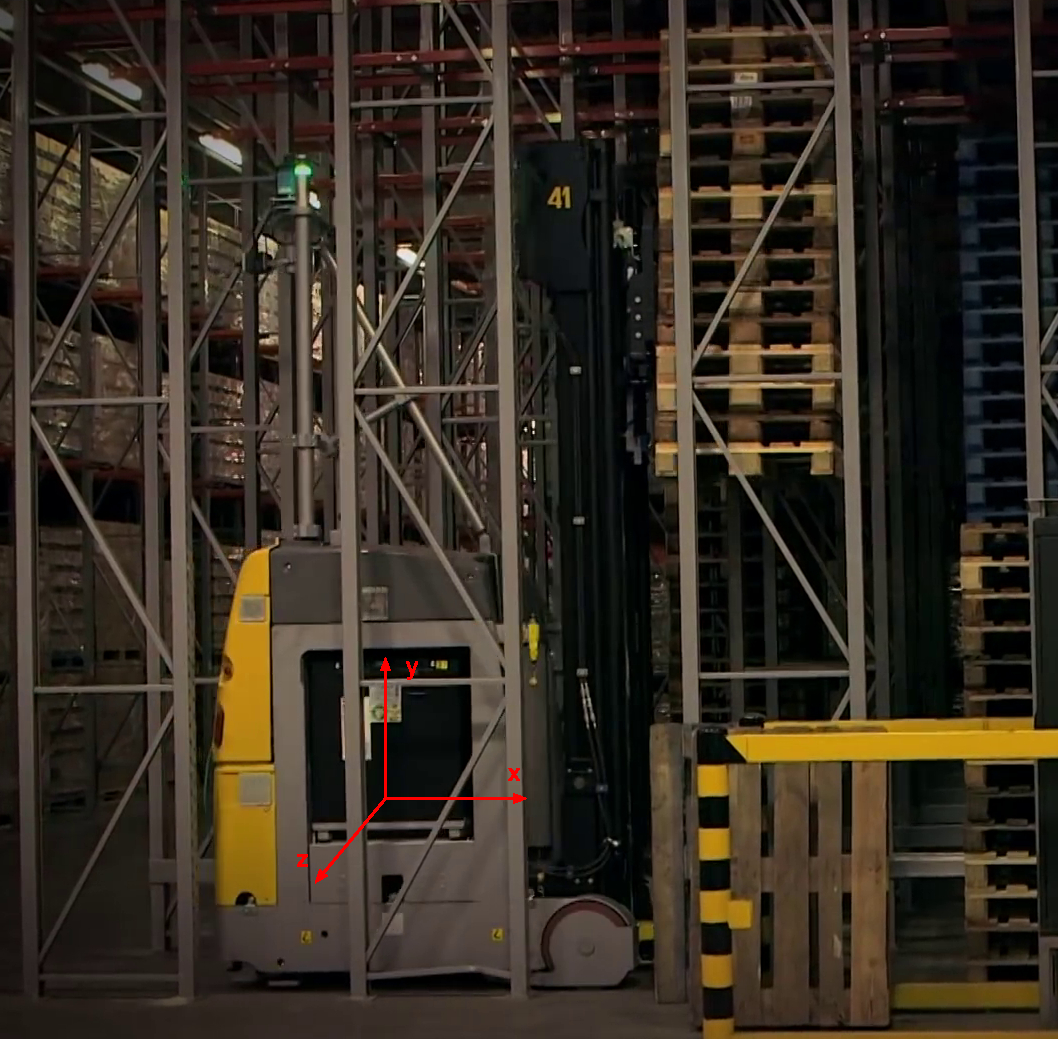
\includegraphics[width=\textwidth]{Img/LGV/op_po}
		\end{center}
	\end{columns}
\end{frame}

\begin{frame}
	\frametitle{Individuazione manuale dei Punti Operazione}
	\begin{columns}
		\column{0.6\textwidth}
			\begin{large}
				\begin{itemize}
					\item Misurazioni manuali sul campo
					\begin{itemize}
						\item Si guida manualmente un veicolo nel magazzino
						\item Una volta individuata una posizione corretta la si registra nel database
						\item Difetti:
							\begin{itemize}
								\item Alto costo in ore/uomo
								\item Pu� richiedere un blocco della produzione
							\end{itemize}
					\end{itemize}
					\item Selezione manuale tramite software
					\begin{itemize}	%migliorare linguaggio
						%\item Meno complessa delle misurazioni sul campo
						\item Difetti:
							\begin{itemize}
								\item Pi� lenta di una selezione automatica
								\item Potenzialmente imprecisa e sensibile all'errore umano
							\end{itemize}
					\end{itemize}
				\end{itemize}
			\end{large}
		\column{0.4\textwidth}
		\vskip 0.7cm
		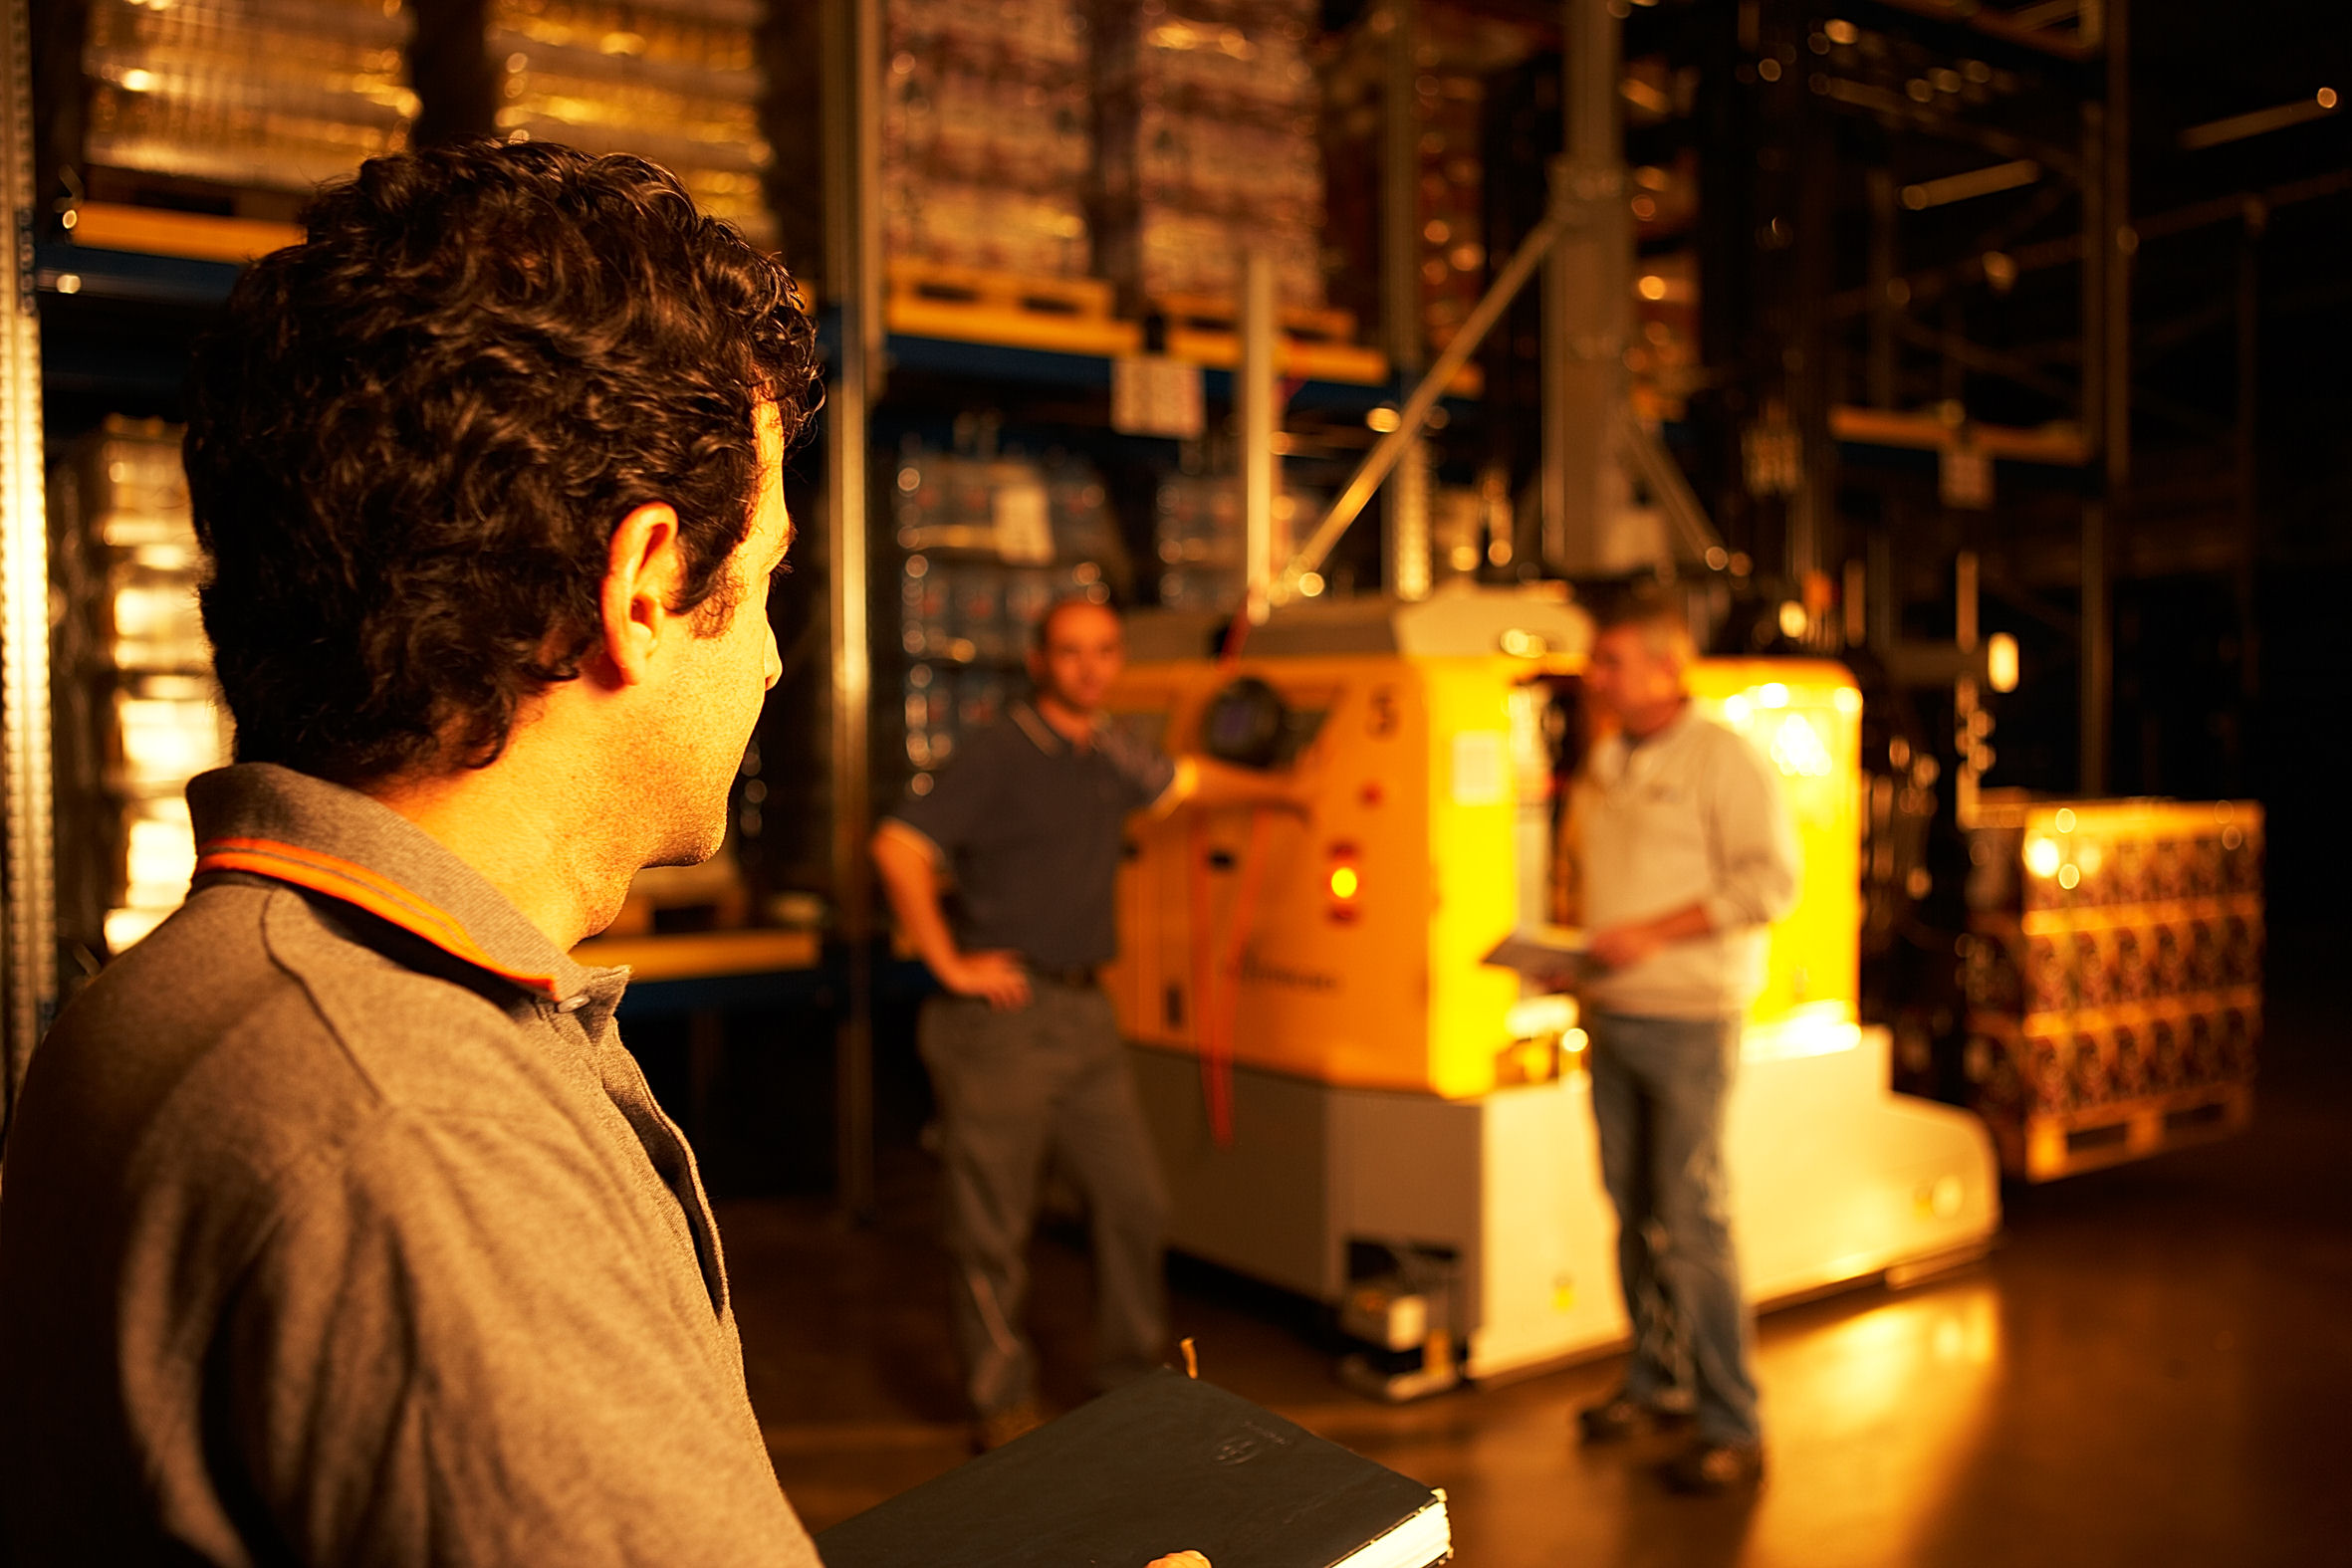
\includegraphics[width=0.8\textwidth]{Img/LGV/indman}\vskip 1.3cm
			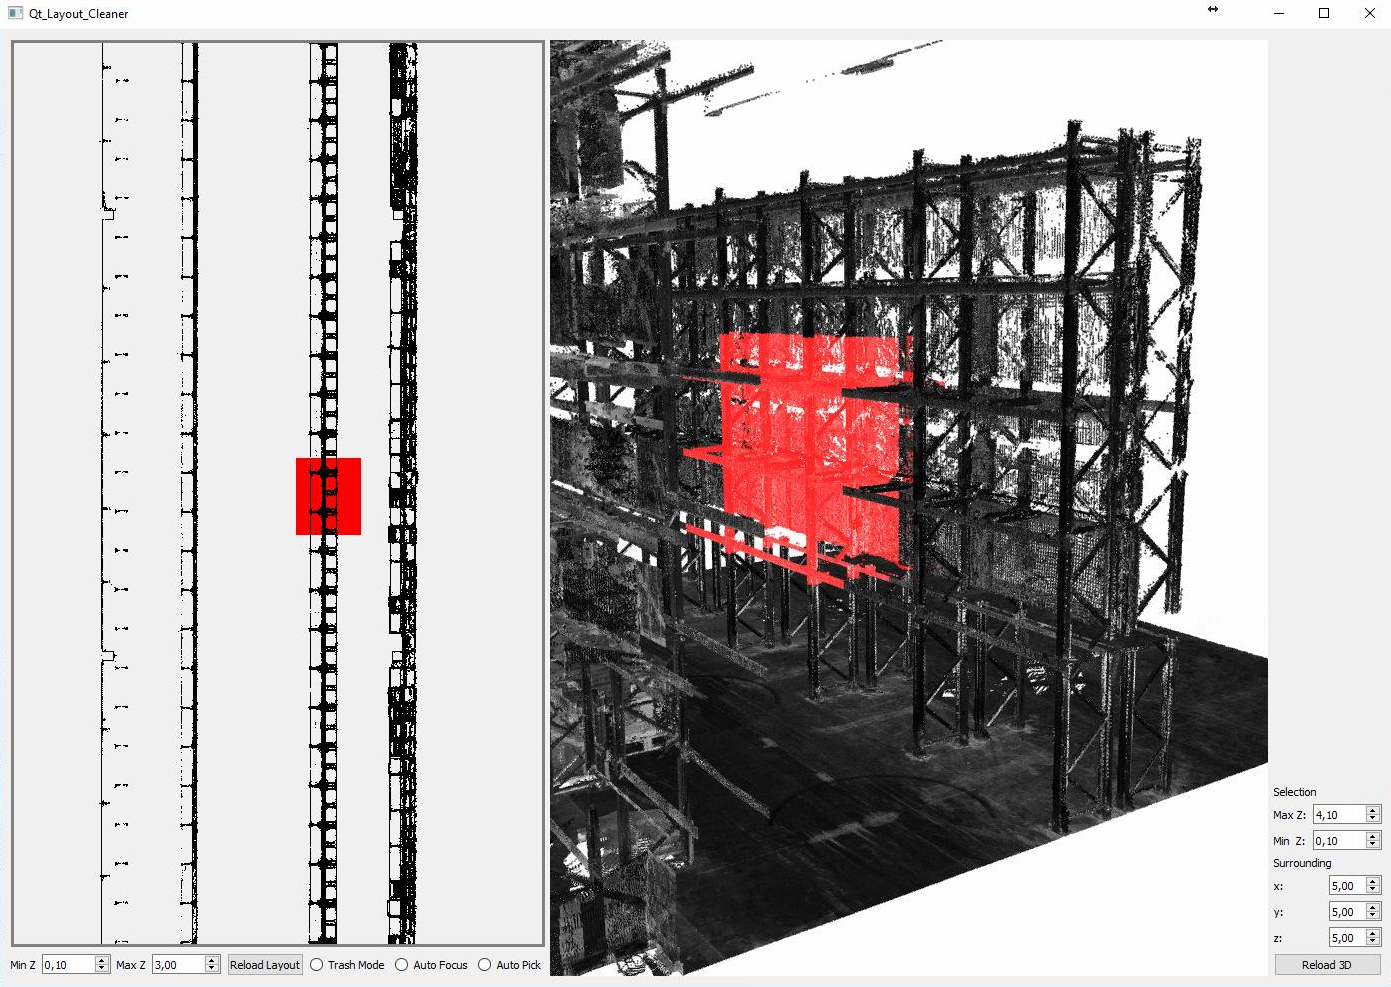
\includegraphics[width=0.8\textwidth]{Img/LGV/select}
	\end{columns}
\end{frame}

\begin{frame}
	\frametitle{Descrizione del sistema sviluppato}
	\begin{columns}
		\column{0.6\textwidth}
		\begin{itemize}
			\item Il sistema esegue una ricerca di tipo pattern matching su un'immagine 2D
			\item Si hanno a disposizione delle scansioni laser terrestri dei magazzini, aquisite con sensori Leica ScanStation P30
			\item I dati in entrata sono sotto forma di Point Cloud (che deve essere convertita in un'immagine 2D)
			\item La Point Cloud di un magazzino medio contiene miliardi di punti
		\end{itemize}
		\column{0.4\textwidth}
		\begin{center}
			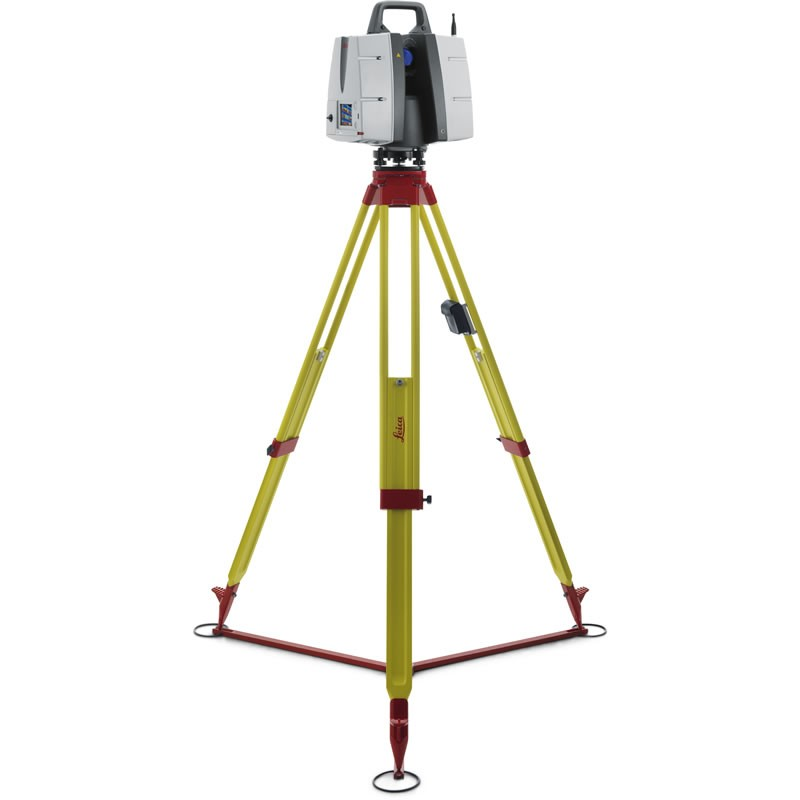
\includegraphics[width=0.7\textwidth]{Img/LGV/Leica_ScanStation_P30}\\
			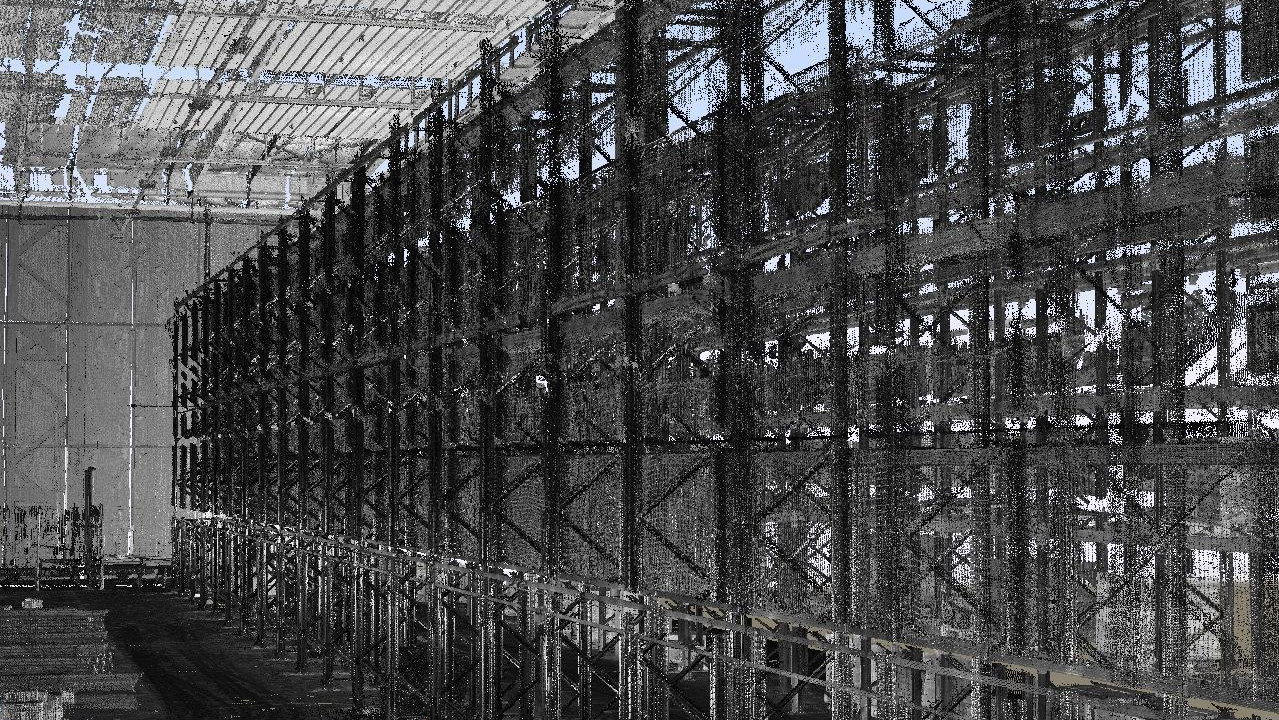
\includegraphics[width=\textwidth]{Img/LGV/pcld}
		\end{center}
	\end{columns}
\end{frame}

\begin{frame}
	\frametitle{Descrizione del sistema sviluppato}
	\begin{columns}
		\column{0.4\textwidth}
		Per convertire una Point Cloud in un'immagine 2D:
			\begin{enumerate}		%must be better
				\item Si assegna un valore ai punti in base alla curvatura della superficie sottostante stimata
				\item Si appiattisce la point cloud e si sommano i valori che cadono sulle celle di una griglia in 2D
				\item Si assegna un colore in scala di grigi alle caselle della griglia in base al colore
			\end{enumerate}
		\column{0.5\textwidth}
			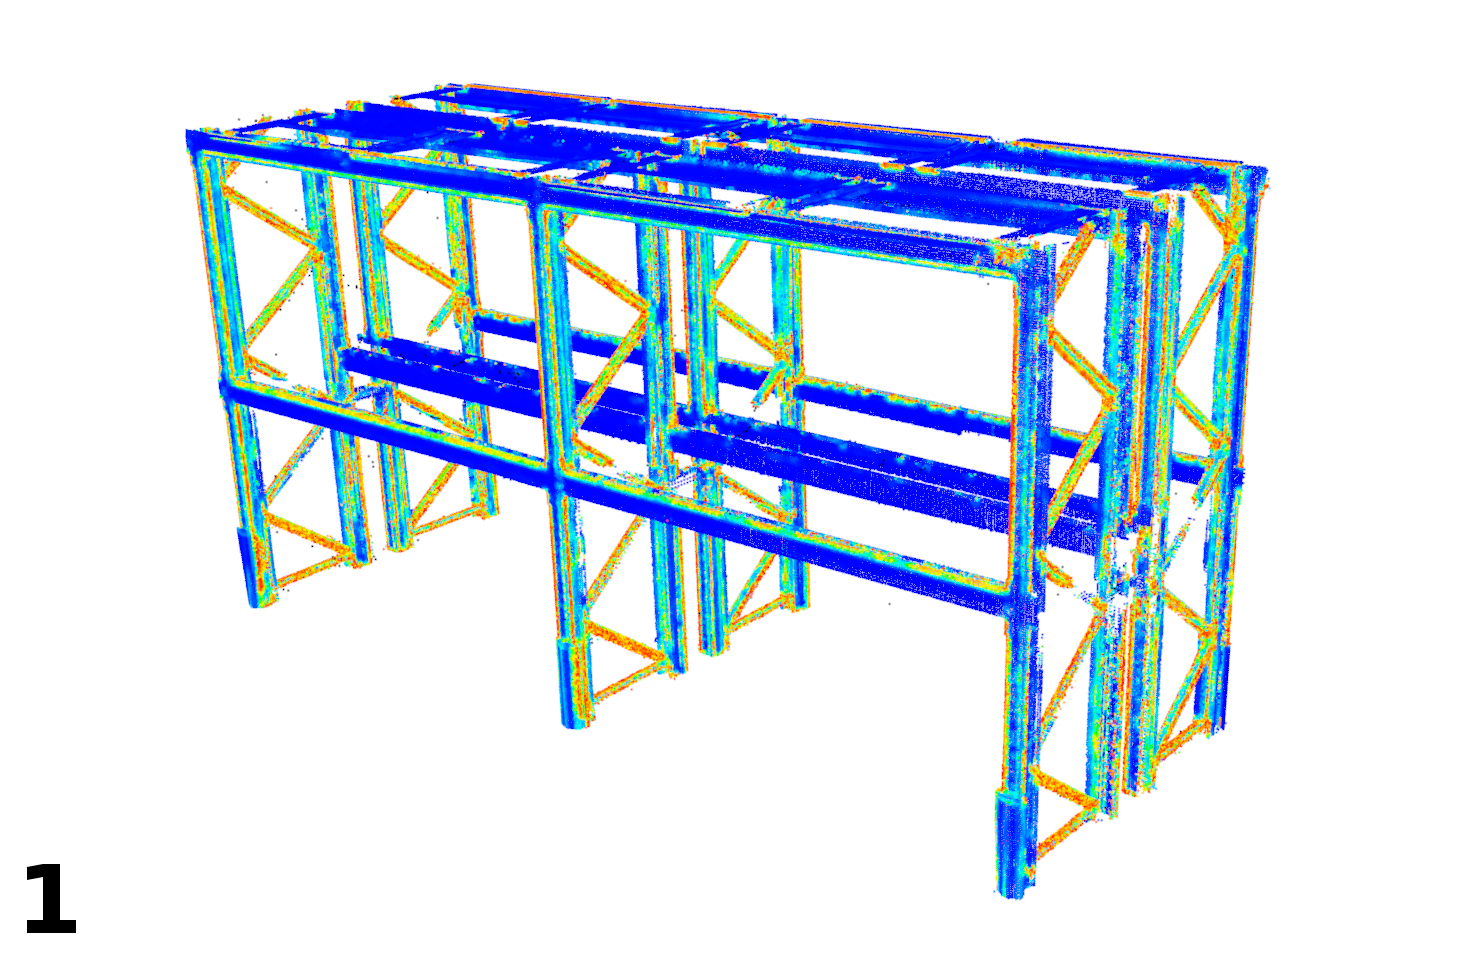
\includegraphics[width=0.6\textwidth]{Img/CURVATURE/CURVATURE_02_num}
			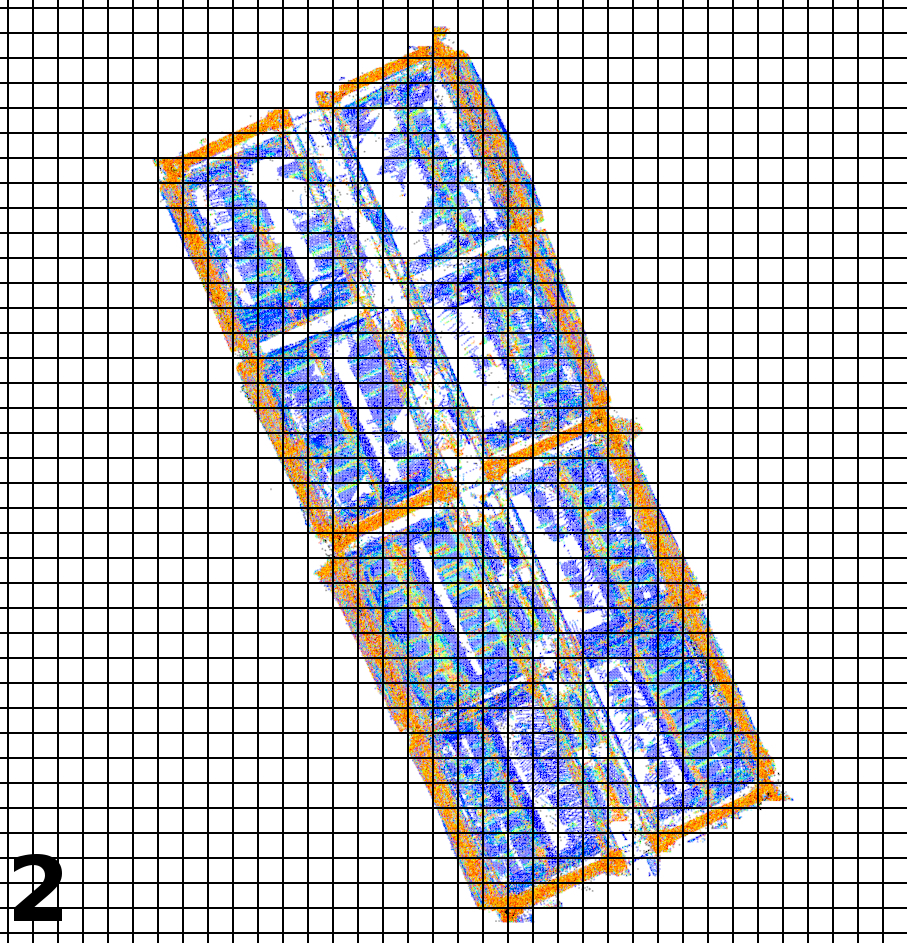
\includegraphics[width=0.4\textwidth]{Img/CURVATURE/CURVATURE_01_grid_num}
			\vskip 0.5cm
			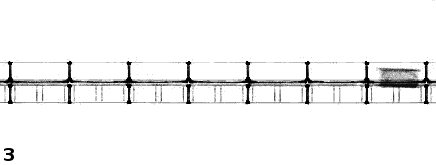
\includegraphics[width=\textwidth]{Img/2D/mag_2d_num_inv}
	\end{columns}
\end{frame}

\begin{frame}
	\frametitle{Descrizione del sistema sviluppato}
	\begin{columns}
		\column{0.5\textwidth}
			\begin{itemize}
				\item La libreria OpenCV assegna un valore ad ogni pixel in base alla somiglianza con un template
				\item Il valore � determinato con una Cross Correlation tra l'immagine e il template
				\item Il template deve essere selezionato dall'utente
				\item Sono necessari alcuni filtri
			\end{itemize}
		\column{0.4\textwidth}
		\begin{center}
			\begin{tiny}
				Template:\vskip 0.3cm
				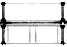
\includegraphics[scale=0.5]{Img/2D/template}
				\vskip 0.5cm Immagine 2D degli scaffali:
				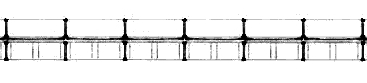
\includegraphics[width=\textwidth]{Img/2D/mag_2d_inv_crop}
				\\Corrispondenze con il template (in azzurro):
				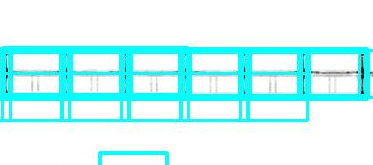
\includegraphics[width=\textwidth]{Img/2D/nofilter_crop_inv}
				\\Risultati filtrati:
				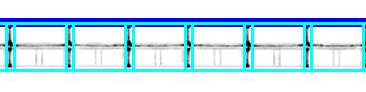
\includegraphics[width=\textwidth]{Img/2D/found_curves_red_crop_inv}
			\end{tiny}
		\end{center}
	\end{columns}
\end{frame}

\begin{frame}
	\frametitle{Descrizione del sistema sviluppato}
	\begin{multicols}{2}
		\begin{itemize}
			\item Soglia
				\begin{itemize}
					\item Scarta i risultati dal valore troppo basso
				\end{itemize}
			\item Non Maximum Suppression
				\begin{itemize}
					\item Elimina le individuazioni multiple dello stesso oggetto
				\end{itemize}
			\item Stima dell'orientamento delle file
				\begin{itemize}
					\item Si ipotizza che gli scaffali siano disposti in file
					\item Scarta i risultati troppo lontani dalle file stimate
				\end{itemize}
		\end{itemize}
	\columnbreak
			\begin{center}
				{\bfseries Soglia alta - individuazione di pochi risultati\\
				$\Downarrow$\\
				Filtro NMS - rimozione dei duplicati\\
				$\Downarrow$\\
				Stima delle file di scaffali con i risultati rimasti\\
				$\Downarrow$\\
				Soglia bassa - si ripete la ricerca\\
				$\Downarrow$\\
				Eliminazione dei risultati troppo lontani dalle file ipotizzate\\
				$\Downarrow$\\
				Filtro NMS - eliminazione dei duplicati rimanenti}
			\end{center}
	\end{multicols}
\end{frame}

\begin{frame}
\frametitle{Risultati su un magazzino completo}
\vskip -0.5cm
\begin{itemize}
	\item La linea blu rappresenta la fila di scaffali ipotizzata dal sistema
	\item Si pu� osservare un falso positivo che � sfuggito ai filtri, a sinistra nell'immagine
\end{itemize}
\vskip 0.5cm
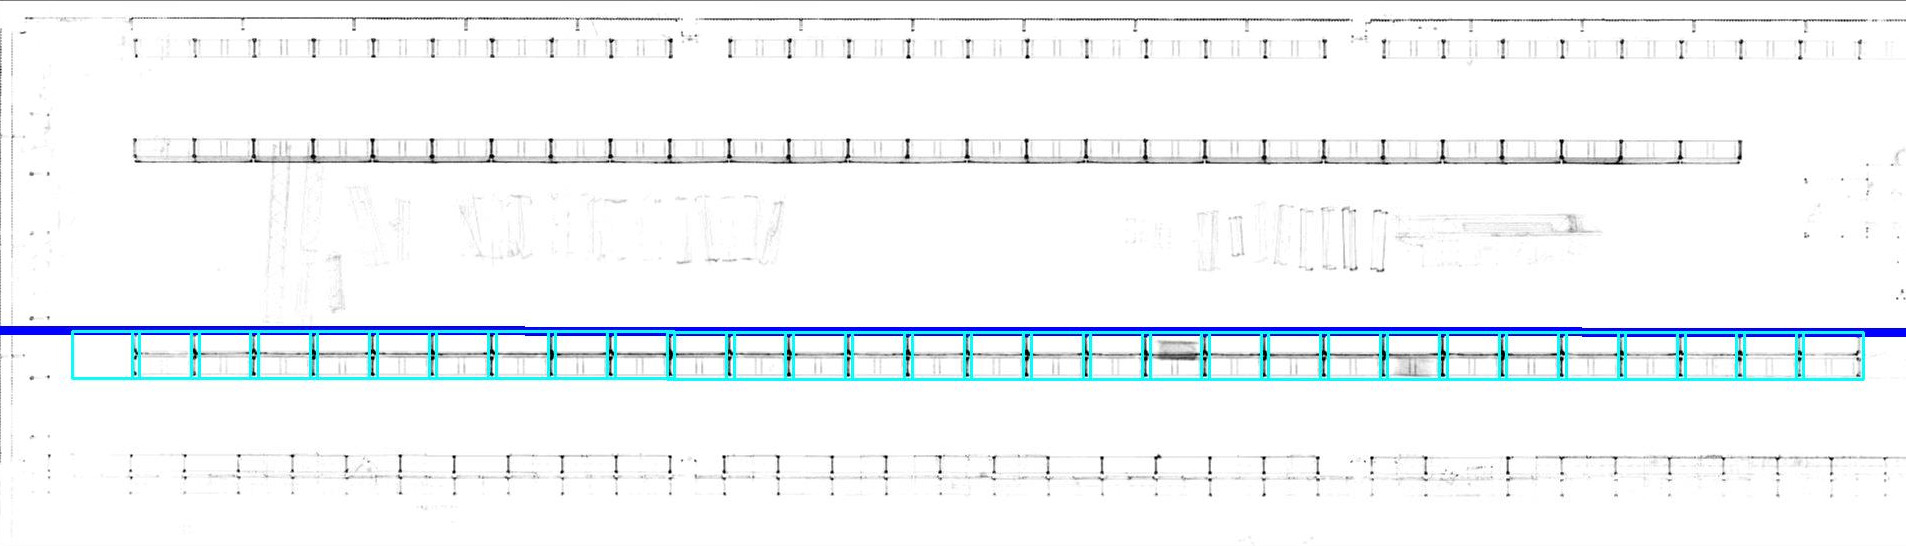
\includegraphics[width=\textwidth]{Img/2D/found_curves_red_inv}
\end{frame}

\begin{frame}
\pgfplotsset{width = \textwidth}
	\frametitle{Risultati statistici}
	\begin{columns}
		\column{0.6\textwidth}
		
		\begin{itemize}
			\item Mediamente il sistema trova quasi tutti gli oggetti cercati ma genera spesso qualche falso positivo
			\item Correggere un falso positivo � preferibile a correggere un falso negativo
			\item I tempi di generazione dell'immagine 2D sono inferiori a un'ora su un magazzino di $95m\times27m$
			\item Una volta generata l'immagine, la ricerca richiede pochi minuti sul magazzino mostrato
		\end{itemize}
		
		\column{0.4\textwidth}
		\begin{center}
			\begin{tiny}
				Dati ottenuti da test svolti con diversi orientamenti delle file di scaffali:\vskip 0.3cm
				\begin{tikzpicture}
					\begin{axis}[
						ybar,
						enlargelimits=0.15,
						legend style={at={(0.5,-0.2)},
							anchor=north,legend columns=-1},
						ylabel={Falsi positivi/Totale (\%)},
						symbolic x coords={-20\degree,-10\degree,0\degree,%
							10\degree,20\degree,180\degree},
						xtick=data,
						nodes near coords,
						nodes near coords align={vertical},
						]
						\addplot[draw=gray, fill=gray, bar width=0.06\textwidth] coordinates {
							(-20\degree,1.3) (-10\degree,0.3) (0\degree,4.5)
							(10\degree ,0.3) (20\degree,3.5) (180\degree,2.4)
						};
					\end{axis}
				\end{tikzpicture}
				\begin{tikzpicture}
					\begin{axis}[
						ybar,
						enlargelimits=0.15,
						legend style={at={(0.5,-0.2)},
							anchor=north,legend columns=-1},
						ylabel={Numero medio di falsi positivi},
						symbolic x coords={-20\degree,-10\degree,0\degree,%
							10\degree,20\degree,180\degree},
						xtick=data,
						nodes near coords,
						nodes near coords align={vertical},
						]
						\addplot[draw=gray, fill=gray, bar width=0.06\textwidth] coordinates {
							(-20\degree,0.5) (-10\degree,0.2) (0\degree,2.6)
							(10\degree ,0.2) (20\degree,1.1) (180\degree,1)
						};
					\end{axis}
				\end{tikzpicture}
			\end{tiny}
		\end{center}
	\end{columns}
\end{frame}

\begin{frame}
	\frametitle{Limitazioni}
	\begin{columns}
		\column{0.6\textwidth}
		\begin{itemize}
			\item La scelta del template pu� influenzare i risultati
			\item Il filtro NMS a volte elimina risultati corretti
			\item La funzione che stima le file di scaffali � inefficace se gli scaffali non sono in fila
			\item Al momento il sistema non trova scaffali simili al template ma orientati diversamente
			\item Non � stato possibile verificare sul campo il livello di precisione dei dati ottenuti
		\end{itemize}
		\column{0.4\textwidth}
		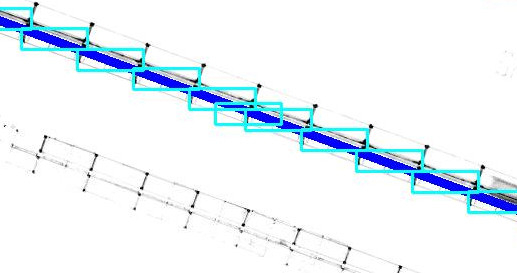
\includegraphics[width=\textwidth]{Img/2D/aberrazioni_crop_inv}\\
		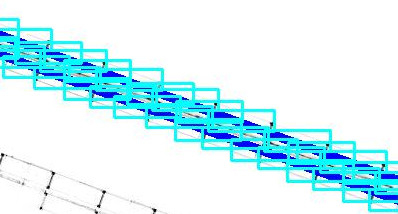
\includegraphics[width=\textwidth]{Img/2D/aberrazioni0_crop_inv}
	\end{columns}
\end{frame}

\begin{frame}
	\frametitle{Sviluppi futuri}
		\begin{center}
			\begin{large}
				\begin{itemize}
					\item Ricerca di oggetti orientati diversamente dal template
					\item Miglioramenti del filtro NMS
					\item Verifica sul campo della correttezza dei risultati ottenuti
					\item Integrazione del sistema nella progettazione di magazzini automatizzati
				\end{itemize}
			\end{large}
		\end{center}
\end{frame}

\begin{frame}
	\frametitle{Grazie}
	\begin{center}
		\vskip 3cm
		\begin{huge}
				Grazie per l'attenzione!
		\end{huge}
		\vskip 3cm
		Giorgio Ghisotti\\
		giorgio.ghisotti@studenti.unipr.it
	\end{center}
\end{frame}


























\end{document} 